%%%%%%%%%%%%%%%%%%%%%%%%%%%%%%%%%%%%%%%%%%%%%%%%%%%%%%%
%                File: OpEx_temp.tex                  %
%                  Date: Sept. 2, 2009                %
%                                                     %
%           LaTeX template file for use with          %
%           OSA's journal Optics Express              %
%                                                     %
%  send comments to Jennifer Mayfield, jmayfi@osa.org %
%                                                     %
% This file requires style file, opex3.sty, under     %
%              the LaTeX article class                %
%                                                     %
%   \documentclass[10pt,letterpaper]{article}         %
%   \usepackage{opex3}                                %
%                                                     %
% Note that our online submission system does not     %
% currently process PDFLaTeX; if PDFLaTeX must be     %
% used, pls. contact OpEx staff, and we will process  %
% manually                                            %
%                                                     %
%                                                     %
%       (c) 2009 Optical Society of America           %
%%%%%%%%%%%%%%%%%%%%%%%%%%%%%%%%%%%%%%%%%%%%%%%%%%%%%%%

%%%%%%%%%%%%%%%%%%%%%%% preamble %%%%%%%%%%%%%%%%%%%%%%%%%%%
\documentclass[10pt,letterpaper]{article}
\usepackage{{../lib/opex3}}
%\usepackage{{../lib/penarandaY}}
\graphicspath{{../Pictures/}}
\usepackage{caption}
\usepackage{subcaption}
\usepackage{amsmath} % Required for equation and aligned environments
\usepackage{hyperref}
\RequirePackage{numprint}

%\usepackage{ae} %%for Computer Modern fonts

%%%%%%%%%%%%%%%%%%%%%%% begin %%%%%%%%%%%%%%%%%%%%%%%%%%%%%%
\begin{document}

%%%%%%%%%%%%%%%%%% title page information %%%%%%%%%%%%%%%%%%
\title{Chromatic Objective Optimization for Extended Depth of Focus \textit{(EDOF)}}

\author{M. Gostiaux Gabriel, M. Yohan Penaranda}

\address{M. Gabriel Gostiaux, Master of Science student, Institute of Optics, \\ Palaiseau, 91 120, France}

\email{gabriel.gostiaux@institutoptique.fr} %% email address is required

\address{M. Yohan Penaranda, Master of Science student, Institute of Optics, \\ Palaiseau, 91 120, France}

\email{yohan.penaranda@institutoptique.fr} %% email address is required

%\homepage{https://github.com/GabrielGst?tab=repositories} %% author's URL, if desired

%%%%%%%%%%%%%%%%%%% abstract and OCIS codes %%%%%%%%%%%%%%%%
%% [use \begin{abstract*}...\end{abstract*} if exempt from copyright]

\begin{abstract*}
This study introduces optimization through optical design softwares such as Zemax Optic Studio to basic concepts of co-design. The optimization can be monitored with matlab via the Zemax OS API, in order to optimize parameters of a chromatic imaging system dedicated to EDOF. In the end, the image will be post-processed using high-frequency transfer algorithm to enhance RGB image resolution.
\hfill \break

\textbf{Keywords:} EDOF, high frequency transfer, chromatic imaging system, Zemax OS API, Matlab.


\end{abstract*}

%\ocis{(000.0000) General.} % REPLACE WITH CORRECT OCIS CODES FOR YOUR ARTICLE

%%%%%%%%%%%%%%%%%%%%%%% References %%%%%%%%%%%%%%%%%%%%%%%%%
\begin{thebibliography}{99}

%\bibitem{labwork} F. Goudail, D. Bloch, O. Leveque, ``FED labworks and projects,'' IOGS {\bf lab 3-4-5,} (2024)
\bibitem{trouve} P. TROUVE, ``Co-conception pourr la mesure 3D,'' IOGS, 11--25 (2024).
\bibitem{TNT+08} C.L. Tisse, H.P. Nguyen, R. Tessières, M. Pyanet, and F. Guichard. ``Extended
depth-of-field (EDoF) using sharpness transport across colour channels,'' In
Society of Photo-Optical Instrumentation Engineers (SPIE) Conference Series, {\bf volume 7061, page 4} (2008).

\end{thebibliography}

%%%%%%%%%%%%%%%%%%%%%%%%%%  body  %%%%%%%%%%%%%%%%%%%%%%%%%%
\section{Introduction}
One of the many objectives of co-design is to simulate optical designs in order to optimize costs through reducing the number of elements of the optical chain of a system. It is also possible to replace costly elements with hybrid ones, integrating signal and image processing in the system.

Here, we will focus on system modelling and optimization. In the first section we will see how using an optical design software helps with the modelling of such a chromatic system. We will see how optimizing the curvature radius and the focus, can be monitored by the criteria of maximizing the range within which at least one of the channels is resolved. Again, this is actually equivalent to maximizeing the union of the depth of focus of the three RGB channels of a chromatic camera within a range of interest. Thhis generalized depth of focus (GDOF) will be computed in matlab through the Zemax OS API.  In the second section we will dive into the optimization of the chromatic system in the purpose of using it with the HFR algorithm. Thus, we will optimize it so that each channel have the best Modulation Transfer Function (MTF).

\section{Design simulation}

We work with the file \texttt{add-on-zemax.zmx} which provides a simple design, composed of an add-on and a paraxial lens. The add-on is composed of two different type of glass, separated by a spherical surface of radius $R$. It is this surface that will be optimized later on. The layout is presented on Fig. \ref{fig:layout}, and the chromatic aberration can already be seen to the experimented eye.

\begin{figure}[h]
	\centering
	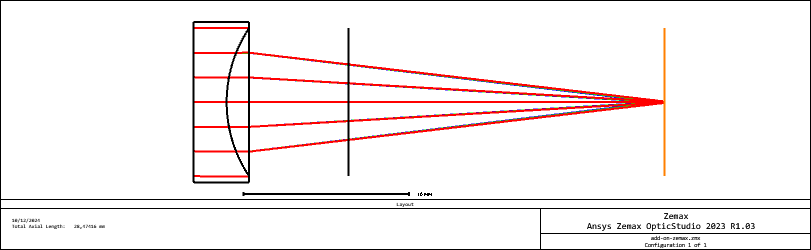
\includegraphics[scale=0.45]{Layout.png}
	\caption{System layout}
	\label{fig:layout}
\end{figure}

We presented the analysis made with the tools provided by Zemax, the through focus spot diagram (TFSD) on Fig. \ref{sub@fig:through-focus} and the longitudinal aberration on Fig. \ref{sub@fig:lon-abe}. The TFSD is interesting because one can see the different focusing planes and the remaining RMS spot size of the other channels in those planes. On the longitudinal aberration, one can observe the focal shift of each channel when variating the field (y axis is the pupil coordinate).

\begin{figure}[h]
    \centering
    \subfloat[Through Focus Spot Diagram]{
        \centering
        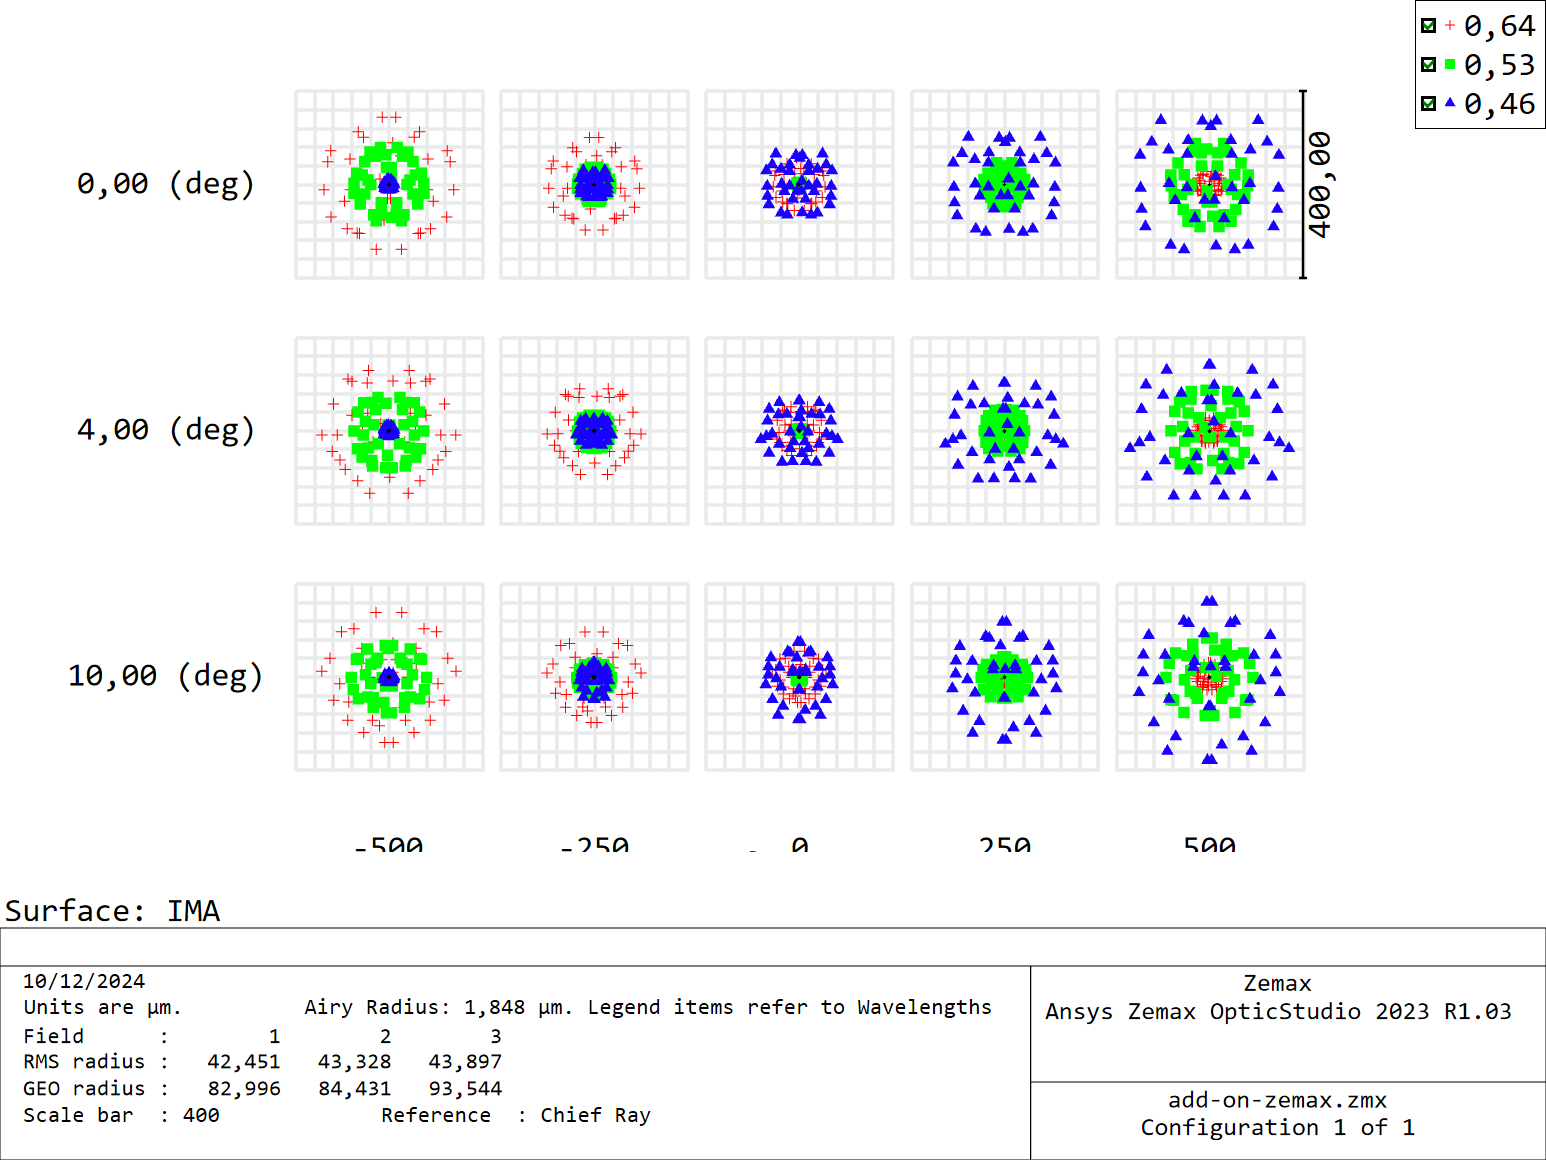
\includegraphics[width=0.3\textwidth]{ThroughFocusSpotDiagram.png}
        \label{fig:through-focus}
    }
	\subfloat[Longitudinal Aberration]{
		\centering
        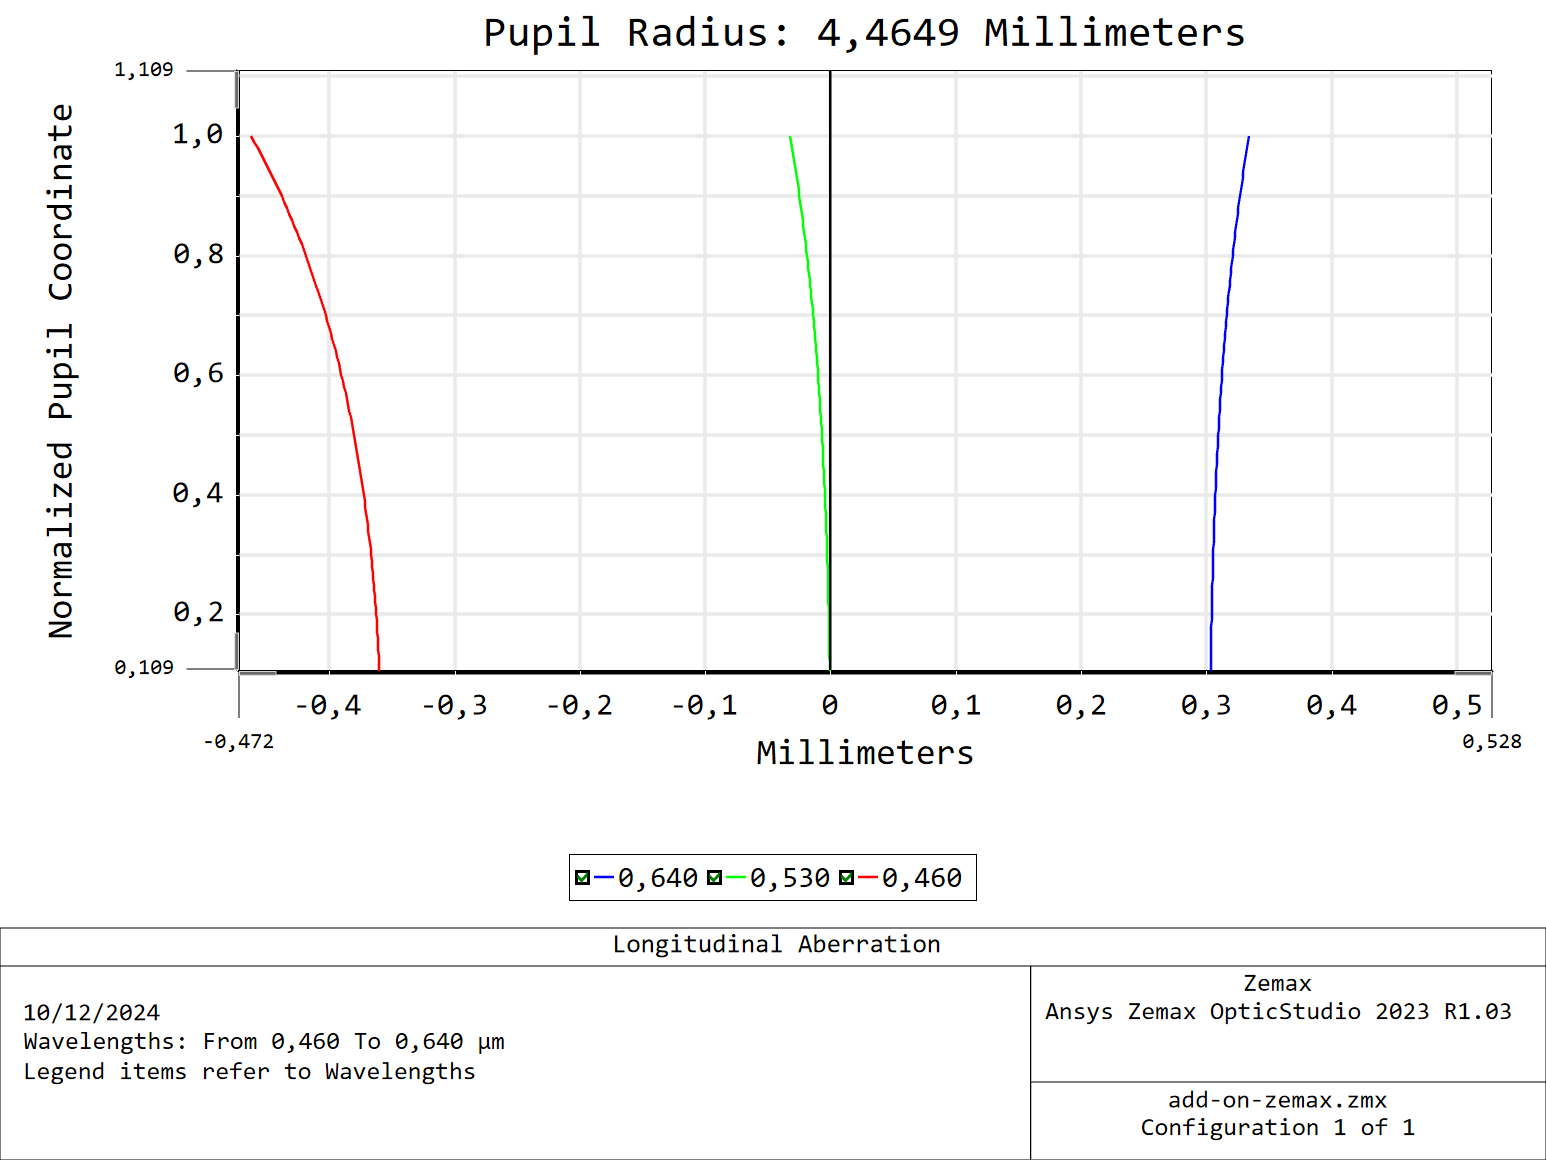
\includegraphics[width=0.3\textwidth]{LongitudinalAberration.png}
        \label{fig:lon-abe}
    }
	\caption{Chromatic aberration of the initial system}
\end{figure}

Thanks to thoses analysis, we can have a first estimate of the chromatic aberration : the longitudinal aberration is $\numprint[mm]{0.68}$ and this is confirmed by the geometric MTF computed with Zemax, as can be seen on Fig. \ref{fig:fft-colors}.
\begin{figure}[h]
    \centering
    \subfloat[MTF (Blue channel)]{
        \centering
        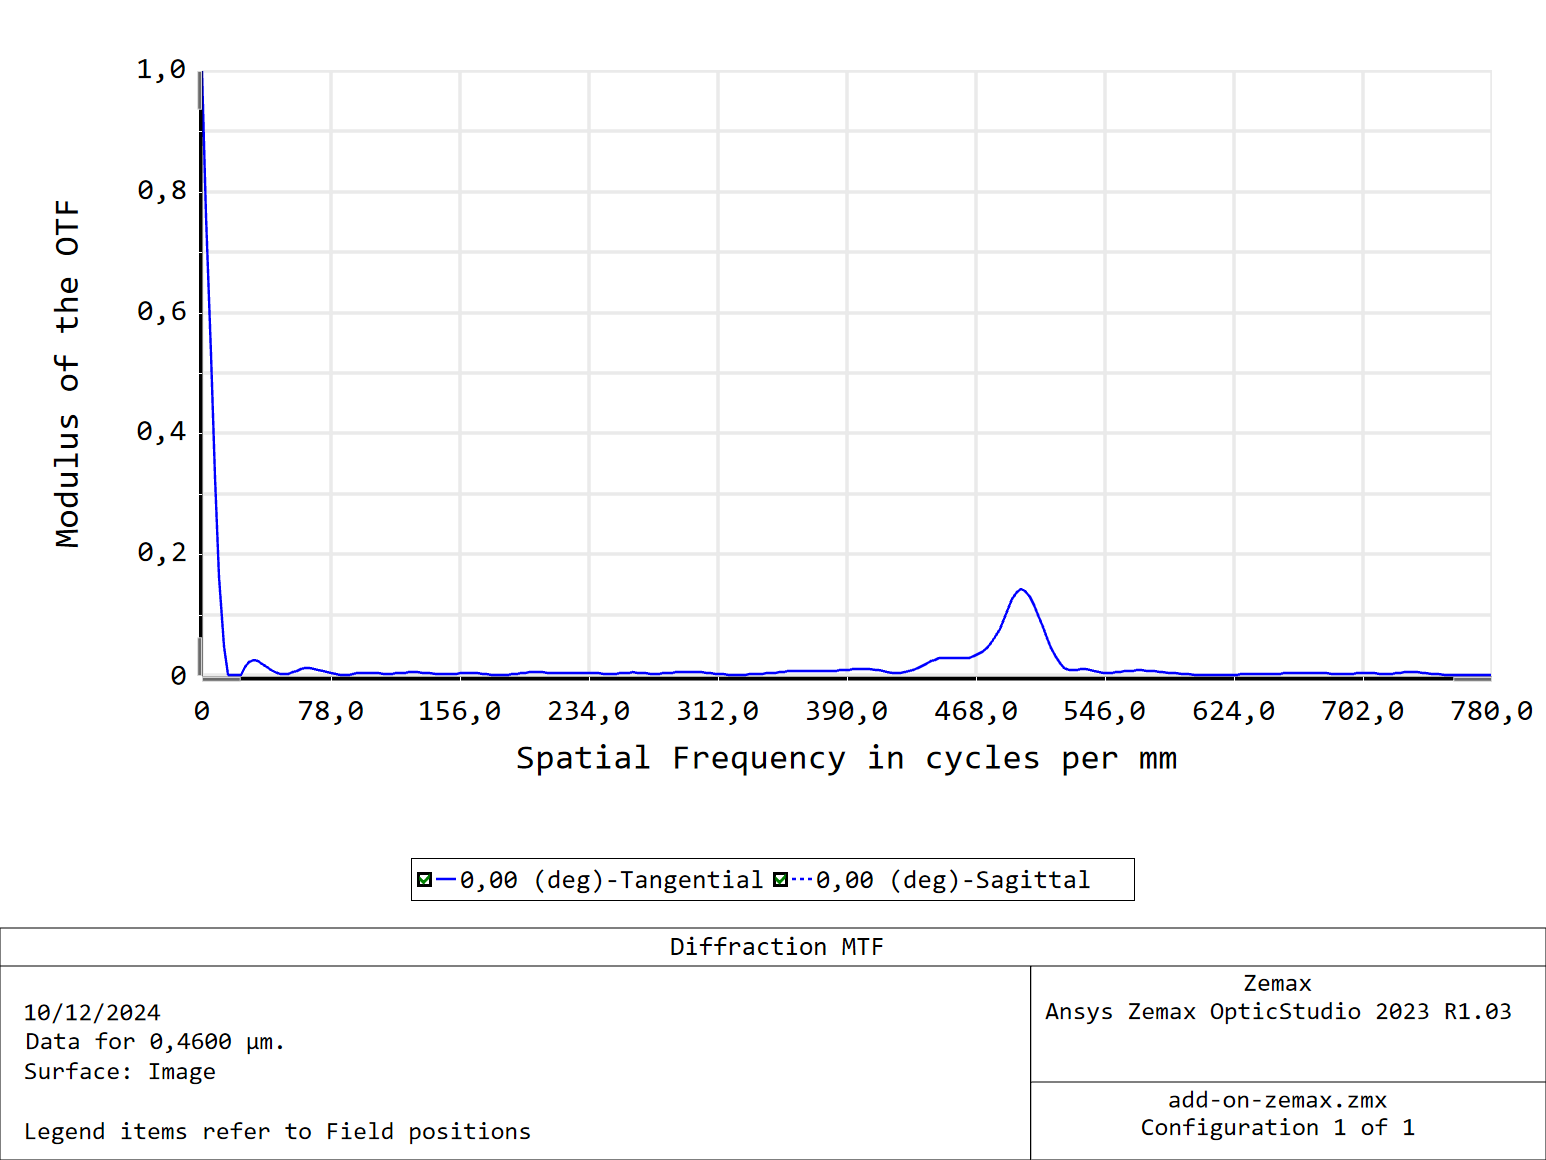
\includegraphics[width=0.3\textwidth]{FFTMTF_blue.png}
        \label{fig:fft-blue}
    }
	\subfloat[MTF (Green channel)]{
		\centering
        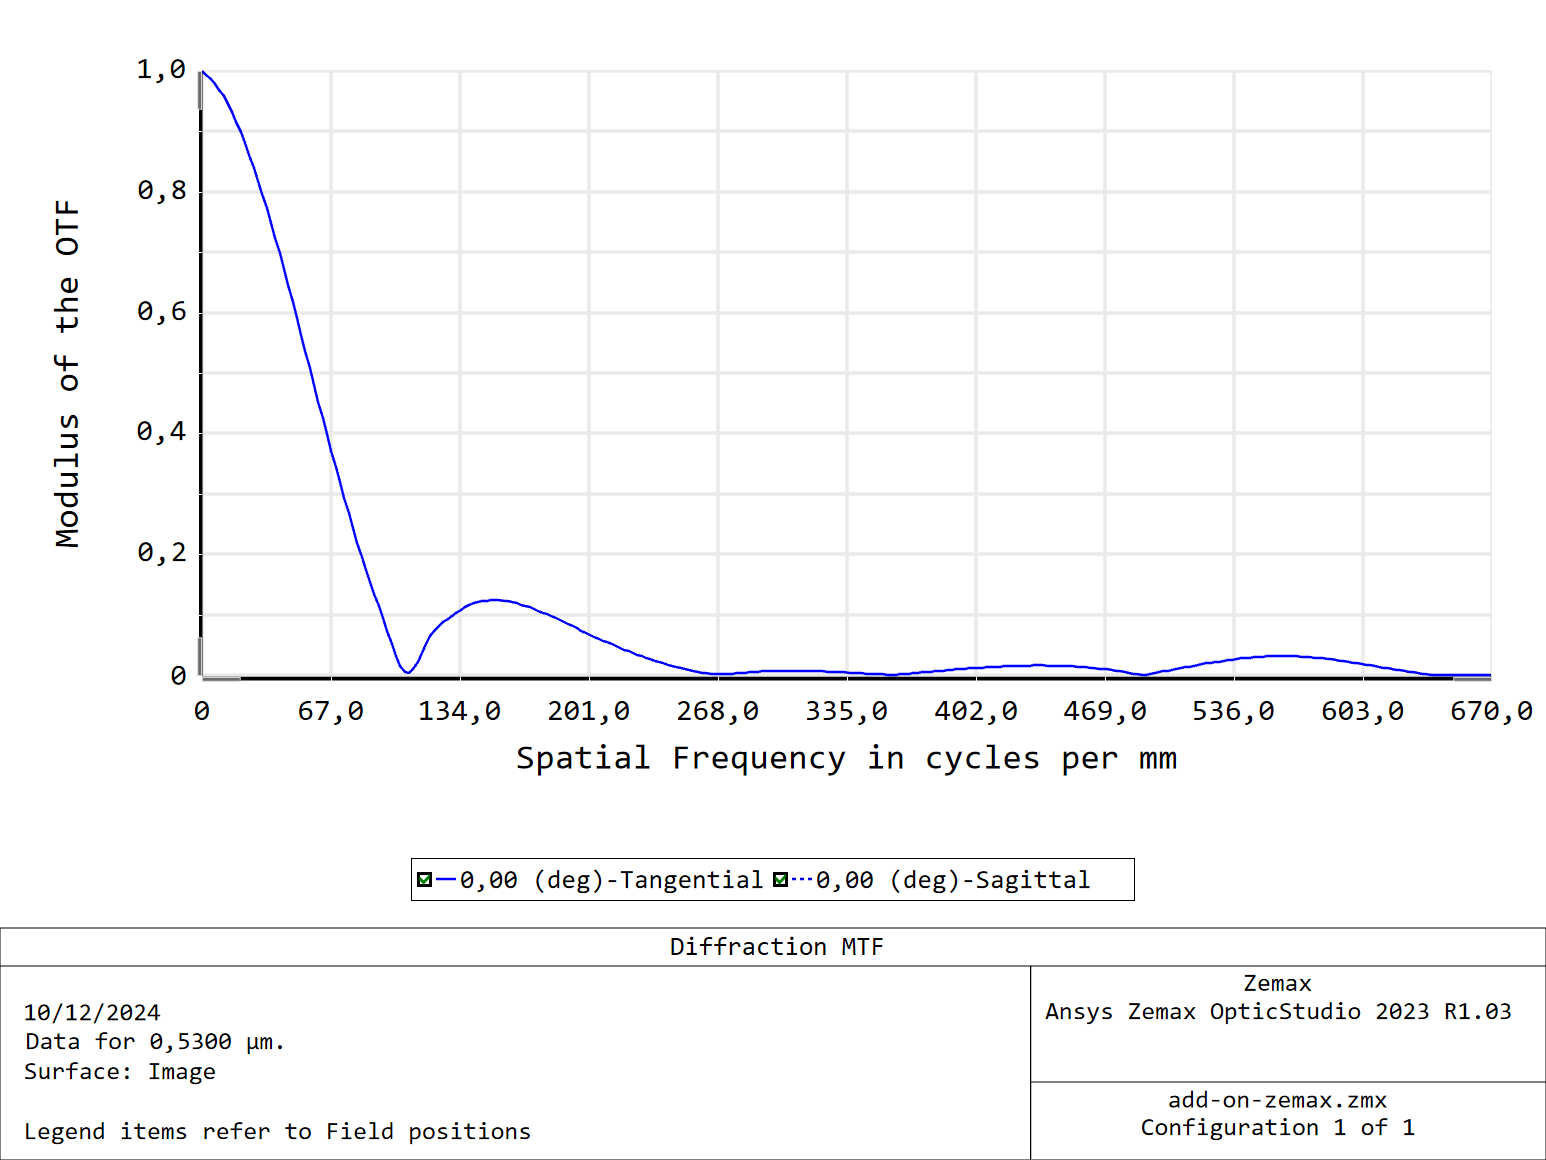
\includegraphics[width=0.3\textwidth]{FFTMTF_green.png}
        \label{fig:fft-green}
    }
    \subfloat[MTF (Red channel)]{
		\centering
        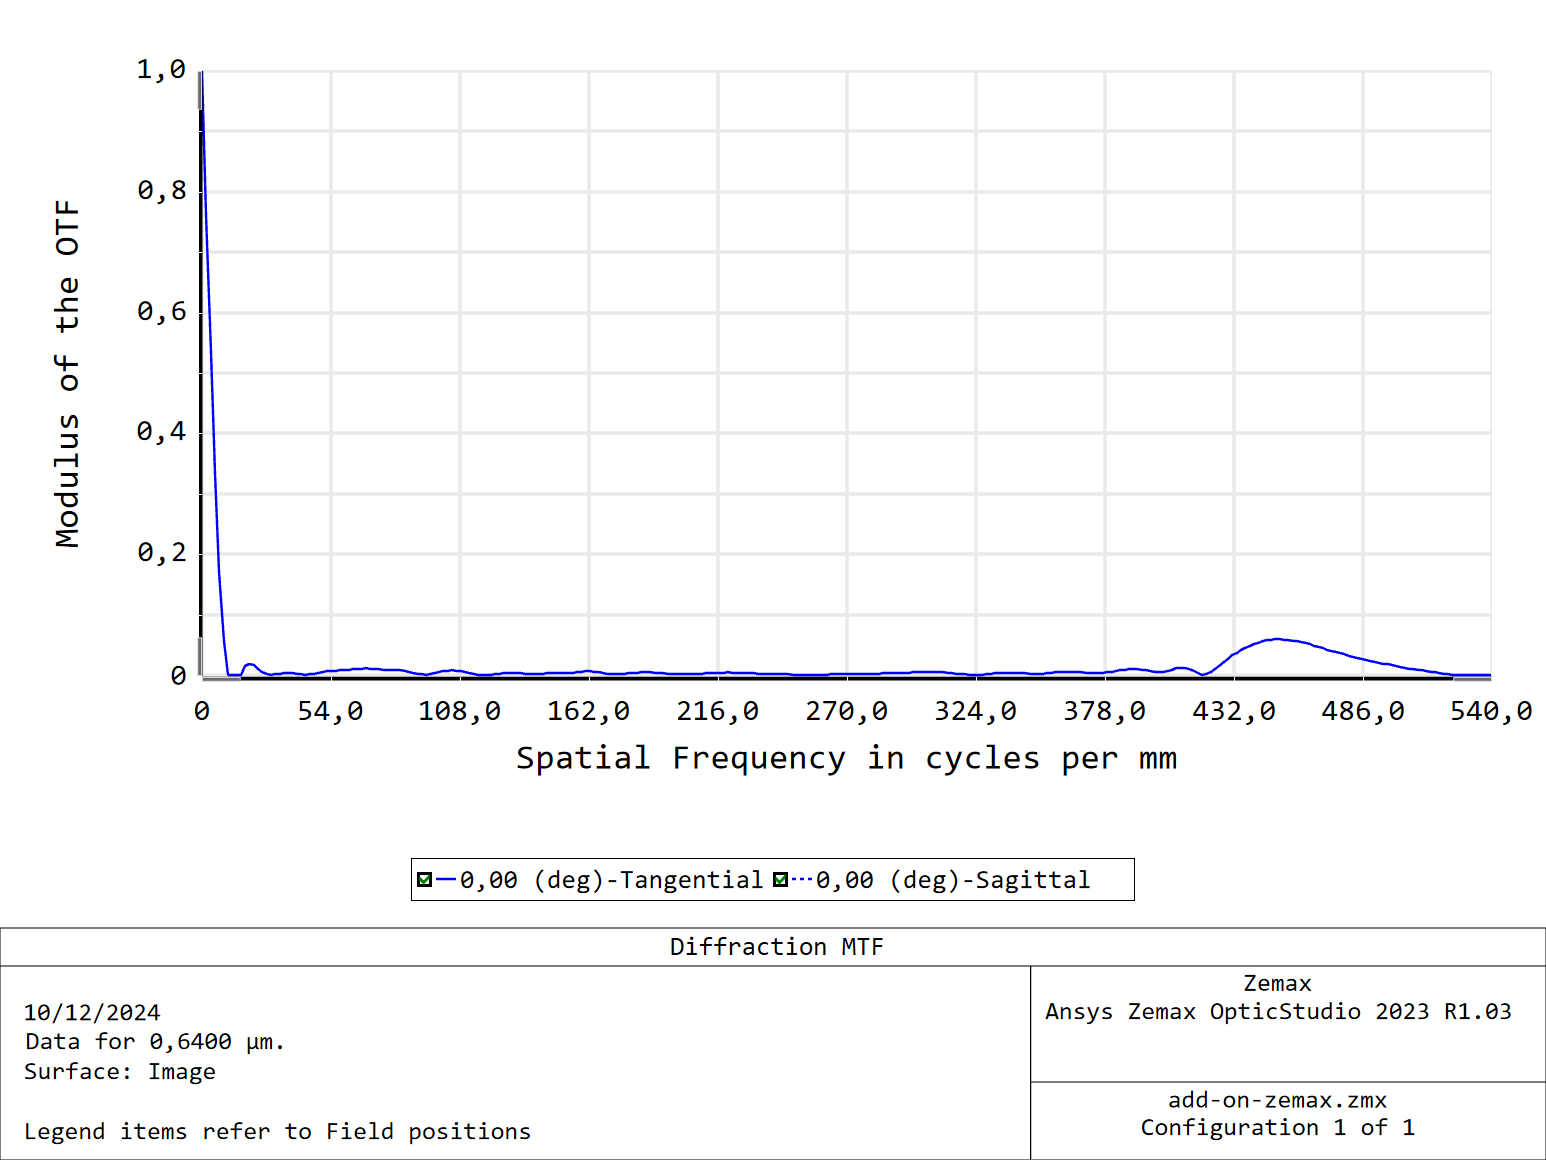
\includegraphics[width=0.3\textwidth]{FFTMTF_red.png}
        \label{fig:fft-red}
    }
	\caption{MTF of different channels }
    \label{fig:fft-colors}
\end{figure}

The sensor position considered in this study is $x'_0 = \numprint[m]{2}$. The Spot Diagram figures allow the extraction of RMS values for different colors. At this position, the RMS radii for red, green, and blue are respectively $RMS_R = \numprint[\mu m]{35.987}$, $RMS_G = \numprint[\mu m]{2.951}$, and $RMS_B = \numprint[\mu m]{37.183}$.
\section{Optimization for HFR post-processing}














\listoffigures

\end{document} 
